% options:
% thesis=B bachelor's thesis
% thesis=M master's thesis
% czech thesis in Czech language
% english thesis in English language
% hidelinks remove colour boxes around hyperlinks

\documentclass[thesis=B,english]{FITthesis}[2012/10/20]

% \usepackage[utf8]{inputenc} % LaTeX source encoded as UTF-8
% \usepackage[latin2]{inputenc} % LaTeX source encoded as ISO-8859-2
% \usepackage[cp1250]{inputenc} % LaTeX source encoded as Windows-1250

\usepackage{graphicx} %graphics files inclusion
% \usepackage{subfig} %subfigures
\usepackage{amsmath} %advanced maths
% \usepackage{amssymb} %additional math symbols
\usepackage{pdfpages}
\usepackage{fancyvrb}

\usepackage{dirtree} %directory tree visualisation


\department{Department of Software Engineering}
\title{Phishing Email Detection based on Entity Recognition}
\authorGN{{\v S}imon} %author's given name/names
\authorFN{Let} %author's surname
\author{{\v S}imon Let} %author's name without academic degrees
\authorWithDegrees{{\v S}imon Let} %author's name with academic degrees
\supervisor{Ing. V{\' i}t List{\' i}k}
\acknowledgements{
I~would like to thank my supervisor Ing. V{\' i}t List{\' i}k, without his assistance and guidance this thesis would have not be accomplished.
\par Then I~would like to thank Ing. Michal Bukovsk{\' y} along with his whole Email.cz team in Seznam.cz for letting me work with them and use their data.
\par My thanks also goes to RNDr. Jana Strakov{\' a} at. el for developing Nametag, Named entity recognition solution, I~used in this thesis, and answering my questions.

\par Finally I~want to thank my family and friends for their support trough my whole studies. 

}
\abstractEN{
%background
Phishing is a serious problem that causes a significant financial loss to many companies wolrdwide.  
Current phishing detection methods for Czech language are not satisfactory.
Named entity recognition (NER) was successfully used for phishing email detection in English and other languages.
%intro
\par The goal of this thesis is to use NER to determine target of the potential phishing email and use this information to detect phishing emails. 
%results
We have developed a solution that can detect target of the potential phishing email.
Our solution works well for major phishing targets such as financial and technology organizations.
We have proved that target detection gives a significant amount of information about the email and can be used to detect phishing.

Our recognizer achieved 86.9\% accuracy when using only one feature generated using target detection.
When using only commonly used features the recognizer achieved 97.7\% accuracy.
Adding target based features gave us minor improvement and achieved 98\% accuracy.
%process
\par For Named entity recognition we use Nametag, the state of the art NER for Czech language.
We have trained our own models for Nametag using both original and custom data.
NER is used to recognize organizations in email.
Custom solution is used to map organizations to domains using data from ARES and Firmy.cz. 
Mapped domains are used to determine target of the potential phishing email.
Target and collected historical data about domains is used to generate features for random forest classifier.
Random forest classifier is used to detect whether or not the email is phishing attack.

\par Nametag model was tested against CoNLL2003 shared task on Named entity recognition.
Target detection solution was tested using 2628 emails from Email.cz data.
Finally the phishing detection recognizer was tested using dataset containing 3744 emails from both public and private sources.


}
\abstractCS{
%background
Phishing je v\'{a}\v{z}n\'{y} probl\'{e}m, kter\'{y} zp\r{u}sobuje nezanedbateln\'{e} finan\v{c}n\'{\i} ztr\'{a}ty mnoha organizac\'{\i}m po cel\'{e}m sv\v{e}t\v{e}.
Sou\v{c}asn\'{e} metody pro detekci phishingu pro \v{c}esk\'{y} jazyk jsou nedostate\v{c}n\'{e}.
Rozpozn\'{a}van\'{\i} entit (NER) bylo \'{u}sp\v{e}\v{s}n\v{e} pou\v{z}ito pro detekci phishing email\r{u} v~anglick\'{e}m i jin\'{y}ch jazyc\'{\i}ch.

%intro
C\'{\i}lem t\'{e}to pr\'{a}ce je pou\v{z}\'{\i}t NER pro ur\v{c}en\'{\i} c\'{\i}le potenci\'{a}ln\'{\i}ho phishing emailu a pou\v{z}\'{\i}t tuto informaci k~detekci phishingu.

%results
Vyvinuli jsme re\v{s}en\'{\i} schopn\'{e} detekovat c\'{\i}l potenci\'{a}ln\'{\i}ho phishing emailu.
Na\v{s}e \v{r}e\v{s}en\'{\i} funguje dob\v{r}e pro v\'{y}znamn\'{e} phishing c\'{\i}le jako t\v{r}eba finan\v{c}n\'{\i} a technick\'{e} spole\v{c}nosti.
Dok\'{a}zali jsme, \v{z}e detekce phishing c\'{\i}le je zdrojem cenn\'{y}ch informac\'{\i} o~phishing emailu a m\r{u}\v{z}e b\'{y}t pou\v{z}ita pro detekci phishingu.

N\'{a}\v{s}e \v{r}e\v{s}en\'{\i} pro rozpozn\'{a}n\'{\i} phishingu dos\'{a}hlo 86.9\% \'{u}sp\v{e}\v{s}nosti p\v{r}i pou\v{z}it\'{\i} pouze jedn\'{e} vlastnosti vygenerovan\'{e} pomoc\'{\i} detekce phishing c\'{\i}le.
P\v{r}i pou\v{z}it\'{\i} be\v{z}n\v{e} pou\v{z}\'{\i}van\'{y}ch vlastnost\'{\i} na\v{s}e \v{r}e\v{s}en\'{\i} dos\'{a}hlo 97.7\% \'{u}sp\v{e}\v{s}nosti.
P\v{r}id\'{a}n\'{\i} vlastnost\'{\i} zalo\v{z}en\'{y}ch na detekci phishing c\'{\i}le zp\r{u}sobilo mal\'{e} zlep\v{s}en\'{\i}. Re\v{s}en\'{\i} dos\'{a}hlo 98\% \'{u}sp\v{e}\v{s}nosti.

%process
Pro rozpozn\'{a}v\'{a}n\'{\i} entit jsme pou\v{z}ili Nametag, sou\v{c}asn\v{e} nep\v{r}ekonan\'{y} NER pro \v{c}esk\'{y} jazyk.
Natr\'{e}novali jsme vlastn\'{\i} modely pro Nametag, pou\v{z}ili jsme p\r{u}vodn\'{\i} a vlastn\'{\i} p\v{r}idan\'{a} data.
NER jsme pou\v{z}ili pro rozpozn\'{a}n\'{\i} entit v~emailu.
Pou\v{z}ili jsme vlastn\'{\i} \v{r}e\v{s}en\'{\i} pro mapov\'{a}n\'{\i} jmen organizac\'{\i} na dom\'{e}ny pomoc\'{\i} dat z~ARES a Firmy.cz.
Namapovan\'{e} dom\'{e}ny jsme pou\v{z}ili pro ur\v{c}en\'{\i} c\'{\i}le potenci\'{a}ln\'{\i}ho phishing \'{u}toku.

Model pro Nametag byl otestov\'{a}n proti dat\r{u}m pro \'{u}kol z~CoNLL2003 zab\'{y}vaj\'{\i}c\'{\i} se rozpozn\'{a}v\'{a}n\'{\i}m entit.
Detekce phishing c\'{\i}le byla otestov\'{a}na pomoc\'{\i} 2628 email\r{u} z~dat od Email.cz.
Nakonec jsme na\v{s}e \v{r}e\v{s}en\'{\i} pro detekci phishingu otestovali pomoc\'{\i} datasetu obsahuj\'{\i}c\'{\i}ho 3744 email\r{u} z~ve\v{r}ejn\'{y}ch i neve\v{r}ejn\'{y}ch zdroj\r{u}.
}
\placeForDeclarationOfAuthenticity{Prague}
\keywordsCS{Phishing, strojov{\' e} u{\v c}en{\' i}, email, rozpoznav{\' a}n{\' i} entit, {\v C}esk{\'y} jazyk}
\keywordsEN{Phishing, machine learning, email, Named entity recognition, Czech language}
\declarationOfAuthenticityOption{1} %select as appropriate, according to the desired license (integer 1-6)


\begin{document}

\setsecnumdepth{part}
\chapter{Introduction}
Phishing is a fraudulent technique with the intention of obtaining confidential user data.  Attackers usually create a similar looking website to a legitimate one. Therefore uneducated users may have trouble spotting the difference and can type their credentials into form on malicious website thinking they are dealing with a legitimate one. In such case attacker gains access to their sensitive data such as login information or credit card credentials. Attackers send hypertext links leading to their malicious website using email.

\par Emails containing such links are called phishing emails. Phishing emails are hard to detect because they have varying form and content \cite{wittel2004attacking}. Attackers are using various techniques such as obfuscation and tokenization to fight phishing detection. \cite{wittel2004attacking}. Phishing emails are not usually sent in such volumes as spam. Therefore traditional anti-spam solutions perform poorly at phishing email detection. Various groups of people has successfully managed to use machine learning for phishing email detection.

\par The goal of this thesis is to research possibilities of using Named entity recognition combined with machine learning and develop filter capable of detecting phishing emails using machine learning approach.

\section{Motivation}
There has been over 90 thousand phishing attacks reported just in the December 2016. \cite{falk2016cerias} Phishing emails have caused huge financial loss to various companies worldwide. \cite{apwg}
\par Detection of phishing email is an uneasy task that cannot be entirely solved using conventional programming methods \cite{falk2016cerias}. Many groups of people tried to solve the problem using machine learning with varying results \cite{fette2007learning} \cite{features2006Chandrasekaran} \cite{featuresBasnet2008detection} \cite{refdByIndia}.  

\section{Goal}
The goal of this thesis is to develop a phishing detection solution that is based on Named entity recognition and proves that Named entity recognition can be used to gain a significant amount of information about the potential phishing email.

\par First we need to research state of the art Named entity recognition and phishing detection solutions.
Then we have to choose Named entity recognition solution that is most fit for our purpose.
We will use the chosen solution to extract information from the emails and generate features for phishing email detection.

\par Next step is to develop baseline phishing email detection solution based on previous research and evaluate the performance of this solution.
Then use features generated using Named entity recognition as features for developed phishing email detection solution.

\par Compare the performance of baseline solution and solution with added features. Describe the benefits of using features generated using Named entity recognition.

\par Evaluate and summarize both the process of research an development and the achieved results. Describe the most important accomplishments of this thesis and suggest possible improvements for future work. 



\setsecnumdepth{all}
\chapter{State-of-the-art}
\section{Phishing email types}
Phishing has varying form because attackers are trying to disguise phishing emails so it does not get detected by phishing and spam detectors. This section will give a quick overview of different types of phishing emails.

\subsection{Link-based} 
Link-based phishing emails are one of the most common forms of phishing. Attackers put hypertext link leading to malicious website into the email. This type of phishing email will be main focus of this thesis.
\subsection{Text-based}
Text-based phishing emails are such emails where attackers put forms requesting sensitive user data directly into email itself, effectively getting rid of hypertext link which may help the phishing email go undetected. They usually create the form using either HTML form tags \cite{w3form} or just plain text. We will detect text-based phishing emails in this thesis.
\subsection{Image-based}
Image-based phishing emails are a result of attackers effort to obfuscate the content of their phishing emails with the aim of making it more difficult to detect their attacks. Such emails use images instead of HTML or text. Attackers create an image containing text making it harder for spam filters to discover the content of the email because image processing and on screen character recognition are complicated tasks. Which makes it hard to detect whether email is phishing or not. Such phishing emails are relatively rare and their detection will not be focus of this work.
\subsection{Attachment-based}
Attachment-based phishing mail takes advantage of email attachments and their diverse formats. Email attachment represents another layer of protection from phishing detection. Many possible formats attachment and complexity of used attachment format makes detection more difficult. We will not focus on detection of this type of phishing email.

\section{Phishing detection approaches}
Phishing emails evolve and change with time. Because of attackers changing the phishing emails they are sending, and colossal financial loss caused by phishing, need for more advanced phishing detection techniques is raising. Scientists have been working on different phishing detection methods. Variety of ways how to detect phishing emails has been developed. This section will list and explain some of approaches used for phishing email detection. Most common phishing detection approaches can be divided into two groups.

\subsection{Blacklist-based}
Generally blacklist is a list of entities, people or other subjects that are considered untrustworthy. Blacklist-based methods use database of known phishing domains, links or email addresses and check potential phishing emails against the database. The main weakness of blacklist-based phishing detection is the blacklist itself. You need to keep blacklist up to date or it becomes worthless and even if we keep the blacklist updated we will never be able to detect zero-day phishing emails. Unfortunately domains used for phishing are often relatively new or hacked legitimate ones \cite{almomani2013phishing} which lowers recall \ref{recall} of blacklist based methods. Blacklisting has high precision \ref{precision} because legitimate websites are unlikely to get into the blacklist. In conclusion blacklisting is simple phishing detection method with high precision but low recall. 

\subsection{Machine learning approach}
Machine learning methods use phishing and non-phishing emails to create a classifier for phishing email detection. As well as blacklist-based approach machine learning approach has certain drawbacks. The process of training the classifier is time-intensive and requires the dataset containing both phishing and non-phishing emails. The dataset greatly influences the performance of classifier. Also the implementation of machine learning algorithms is far more complicated than implementation of blacklist-based methods.  

\section{Phishtank}
One example of black-list based solution is Phishtank. Phishtank is a community website that gathers information about confirmed phishing attacks. The information about attacks is publicly available and can be downloaded in many formats. Anyone can sign up and either submit new phishing attacks or verify existing ones. Furthermore Phishtank offers a free API for both non-commercial and commercial use. \cite{phishtank}

\section{Machine learning}
Machine learning is a subfield of computer science that gives computers ability to learn without being explicitly programmed. \cite{friedberg1958learning} Rather than describing the whole subject of machine learning in detail, this section will briefly describe essential parts of machine learning related of thesis to phishing email detection. Machine learning tasks are usually classified into three general categories.

\subsection{Supervised learning}
\par Supervised learning maps input data to desired output. It is trained using annotated data. Supervised learning the main focus of this thesis. Common tasks include classification tasks such as Computer vision, Speech recognition, Optical character recognition, Information retrieval, Document classification and Phishing email detection.

\subsection{Unsupervised learning}
\par Unsupervised learning annotates or finds structure in data. No training and no annotated training data is required. Some minor parts of this thesis will focus on this category. Unsupervised learning includes certain NLP tasks such as word embeddings \cite{word2vec} and Brown clustering.

\subsection{Reinforcement learning}
\par Reinforcement learning is very different from the two previous categories. It involves a computer interacting with dynamic environment. There is no annotated training data. Instead of training data the system is learning trough reward and punishment. This category includes task such as vehicle driving.


\section{Datasets}
Datasets are collections of data. Datasets are crucial part of all machine learning methods used for phishing email detection. Training dataset has huge impact on performance of the resulting phishing email detector. Ideally the dataset should match the real life data otherwise the resulting model may perform poorly when used with real life data despite the fact that it performs well on held-out data from the dataset.

\subsection{SpamAssassin}
SpamAssassin \cite{spamAssassin} is a high performing \cite{fette2007learning} open source spam detection platform. Spam assassin project has gathered a huge amount of emails.   

\par SpamAssassin email corpus is one of most commonly used publicly available datasets for English language \cite{spamAssassinDataset}. SpamAssassin email corpus consists of both spam and ham messages. Messages were either collected from publicly available sources or sent to author of corpus with permission for public use. SpamAssassin email corpus has been used in many works focused on phishing email detection \cite{ultimateFeatureBreakdown} \cite{fette2007learning} \cite{indiaPaperMultiClassifier}

\subsection{Email.cz dataset} \label{emailczdata}
\par Thanks to Email.cz we have access to moderate dataset of emails. Dataset includes both phishing and non-phishing emails from various sources. There is 5472 phishing and about 10 thousand non-phishing emails in the dataset.
\par Phishing emails come from three different sources.
First part is a public dataset that was downloaded from \cite{monkeyDataset} \footnote{Unfortunatelly the link is not working anymore. We do not know if or where it can be downloaded now.} Second part consists of phishing emails reported by Email.cz users. Last little part was obtained from hoax.cz. 
\par Non-phishing emails is a sample of emails collected from traffic.

\par To our knowledge there are no publicly available phishing datasets for Czech language. All Czech emails used in this thesis were taken from Email.cz dataset. 


\section{Evaluation methods}
Evaluation methods are used for establishing how accurately does given machine learning system perform. When looking at two independent systems we need a well-defined measure that will allow us to compare them.  

\subsection{Precision} \label{precision}
Precision represents how many of tagged samples are relevant. Concerning phishing email detection precision is really important because low precision means that a lot of legitimate emails are being tagged as phishing. Precision only measures the quality of the system not the quantity therefore it can't be used for comparison of two systems by itself.

\subsection{Recall} \label{recall}
Recall represents how many of relevant samples were tagged. Concerning phishing email detection low recall means that a lot of phishing emails are not detected. Recall only measures quantity of the system not the quality that's why it can't be used for serious comparison of two systems by itself.

\subsection{F-measure}
F-measure is a combined measure that incorporates precision and recall. It can be used for measuring performance and comparing machine learning systems. F-measure is defined as a harmonic mean of precision and recall.
\[F\_measure = 2 \cdot \frac{precision \cdot recall}{precision + recall} \]


\section{Machine learning in phishing detection}
This section will give a brief overview of chosen machine learning methods that has been already successfully used for phishing email detection in previous works. Tolan at el. \cite{ultimateFeatureBreakdown} has compared a performance of variety of ML methods when used for phishing email detection. 

\subsection{Linear regression}
Linear regression is one of the simplest machine learning methods. It uses simple mathematical functions with precisely tuned parameters to model the phenomenon. Input of the function are decimal numbers representing chosen features of tested email. Output of the function is one decimal number that is used to determine whether the tested email is phishing or not. 
\par According to \cite{abu2007comparison} Linear regression has the best results out of all compared methods. 
    
\subsection{Support vector machine}
Support vector machine (SVM) is one of the most commonly used machine learning method for phishing detection. The principle behind this method is following. Each email is converted to vector in multi dimensional space. The goal is to find a hyperplane that separates phishing and non-phishing emails. 
\par Support vector machines has been successfully used to detect phishing emails by many researchers including
\cite{features2006Chandrasekaran}, \cite{featuresBasnet2008detection}, \cite{featuresMa2009detecting} and \cite{ultimateFeatureBreakdown}.
    
\subsection{Decision trees and Random forest}
Decision trees learning are a simple machine learning method. Feature vector extracted from the email travels from the root to the leaves of the tree. The path trough the tree is determined by conditions in the nodes of the tree. Result is assigned to each leaf.

\par Random forest is a collection of decision trees. Each tree classifies the email independently and the final result is determined by the voting system. 
\par Decision trees are prone to overfitting the dataset. Random forest should prevent overfitting by training each of the trees with randomly selected of features. Random forests were successfully used in \cite{fette2007learning} and \cite{vitListik2015detekce}.
    
\subsection{Neural networks}
Neural networks are popular machine learning method commonly used for various tasks. This method is inspired by actual neural networks. Neural networks consist of neurons that send and accept signals from one another. Bonds between the neurons have different weight. Neurons are usually organized into layers.
\par This method is not widely used for phishing email detection. It was successfully used alongside with other methods in \cite{abu2007comparison} and \cite{featuresBasnet2008detection}.

\section{Features}
Generally speaking features are pieces of information extracted from the raw data presented to recognizer. When considering phishing detection only data that is guaranteed to be present is the email itself. Websites linked from inside of the email may not be working or links might not be present at all. Therefore many features used for phishing detection in state of the art systems rely only on data available directly from the email itself. 

\par Choosing features carefully is on of the most important tasks when designing any machine learning system \cite{ultimateFeatureBreakdown}. Poor choice of features may drastically reduce performance of phishing detection recognizer. There are numerous works that use dozens of features and compare their effect on performance of phishing email detection system such as \cite{ultimateFeatureBreakdown}, \cite{featuresBasnet2008detection}, \cite{fette2007learning}, \cite{featuresMa2009detecting} and \cite{featuresUrl}.

\section{Features for phishing email detection} \label{features}
In 2010 Tolan has extracted 40 features from emails from three different datasets to determine the features that bring the most valuable information for spam and phishing email detection. \cite{ultimateFeatureBreakdown} Some features were carefully selected form previous papers other features were added by author himself. Features that had brought most significant information gain in all three datasets are following.

\subsection{Body richness} \label{bodyrichnes}
Body richness is defined as the total number of words divided by the number of characters in the email body. Body richness formula is shown in formula. Body richness was originally proposed by Chandrasekaran et al. \cite{features2006Chandrasekaran} and it was in the top three most significant features in all three tested datasets in \cite{ultimateFeatureBreakdown}.
\[ bodyRichness = \frac{numberOfWords}{numberOfCharacters} \]

\subsection{Subject richness}
Subject richness is defined as number of words divided by the number of characters in the email subject. Subject richness formula is shown in formula. This feature was one of the top three most significant features in all three tested datasets in \cite{ultimateFeatureBreakdown}.
\[ subjectRichness = \frac{numberOfWords}{numberOfCharacters} \]

\subsection{Number of links}
This feature represents number of links in the body of the email. It was previously used in following papers \cite{fette2007learning} \cite{featuresBergholz2008improved}. This feature has been also used to detect Czech phishing emails in \cite{vitListik2015detekce}.

\subsection{Number of external links}
Number of external links represents number of links in the body of the email with target outside of the email body. This feature was previously used in \cite{featuresBergholz2008improved}. 

\subsection{Number of domains}
Number of domains measures total number of domains in all URLs in the email. This feature was used in \cite{fette2007learning} and \cite{vitListik2015detekce}.

\subsection{Number of characters}
This feature represents number of characters in the body of the email. It was used in \cite{features2006Chandrasekaran} and \cite{vitListik2015detekce}.

\subsection{Body HTML}
Body HTML is a binary feature that is true when HTML is present in the email. Previously used in \cite{fette2007learning} and \cite{vitListik2015detekce}.

\subsection{Maximum number of periods}
This feature measures maximum number of periods present in a link in the email. This feature was previously used in \cite{fette2007learning} \cite{featuresBergholz2008improved}.

\subsection{Number of words}
Number of words represents total number of words in the body of the email. Used in \cite{features2006Chandrasekaran} and also used in \cite{vitListik2015detekce} to detect Czech phishing emails.

\subsection{Advanced features}
Some researchers took experimenting with features even further by extracting advanced features from the email. \cite{indiaPaperMultiClassifier}. Shyni et al. \cite{indiaPaperMultiClassifier} has developed a successful phishing email detector using features such as Named entity recognition, Topic modeling and Image processing. It is clear that using advanced features can improve the performance of the phishing email detector.


\section{Named entity recognition}
Named entity recognition (NER) is a data extraction task that belongs into group of tasks called Natural language processing. The input is unannotated stream of text and the goal of Named entity recognition is to recognize words or chunks of words that are proper names (entities), such as people, organizations and locations. In addition to entities Named entity recognition implementations sometimes extract other information, such as time, date, hypertext links and email addresses.

\par State of the art implementations reach close to human performance with 93.39 F-measure in MUC-7 \cite{muc7} task and 90.80 F-measure on dataset from CoNLL-2003 shared task \cite{stateOfTheArtConll} \cite{conll2003task}.

\subsection{CoNLL-2003 shared task}
Shared task of Conference on Computational Natural Language Learning in 2003 \cite{conll2003} was focused on language-independent Named entity recognition. CoNLL-2003 shared task provided contestants with annotated training and testing data as well as unannotated data and lists of names. One of the challenges for contestants was to incorporate additional provided data into their solutions. 
\par CoNLL-2003 shared task dataset contains four entity types: person, organization, location and misc for entities that do not belong to previous three categories. Entities are non-embedded, non-overlapping and annotated with exactly one label. \cite{stateOfTheArtCzechNER} There are data available for English an German languages. \cite{conll2003task}
\par Despite being almost 13 years old CoNLL-2003 shared task is still being used as standard measurement for comparison of Named entity recognition systems performance. \cite{stateOfTheArtCzechNER} \cite{strakova2017neural} \cite{stateOfTheArtConll} Initial baseline performance for CoNNL-2003 shared task is 59.61 F-measure. Over dozen of teams have participated in the shared task. The best result achieved was 88.76 F-measure \cite{florian2003conll}. Current state of the art Named entity recognition performance on CoNLL-2003 shared task is 90.80 F-measure. \cite{stateOfTheArtConll}

\subsection{Czech Named Entity Corpus} \label{cnec}
For Czech language the Czech Named Entity Corpus is available. CNEC 2.0 is a large corpus of manually annotated Czech sentences. Corpus contains 46 types of named entities. These fine-grained classes are grouped into 7 supertypes: numbers in addresses, geographic items, institutions, media names, artifact names, personal names and time expressions. Entities can be labeled with one or more classes and can be embedded. \cite{cnec}  
\par Czech Named Entity Corpus was originally released together with a Named entity recognition system that achieved 62 F-measure on fine-grained classes and 68 F-measure on supertypes. In 2011 it was outperformed by recognizer that achieved score of 72.94 F-measure on supertypes. \cite{previousCzechNER} Currently the best performing named entity recognizer on Czech Named Entity Corpus is Nametag with 82.82 F-measure. \cite{stateOfTheArtCzechNER}


\section{Nametag}
Nametag is state of the art implementation of Named entity recognition for Czech language. Nametag also achieved score of 89.16 F-measure on CoNLL-2003 shared task dataset which is close to performance of the current state of the art Named entity recognition system for English language. 
\par The recognizer is based on Maximum Entropy Markov Model and a Viterbi \cite{forney1973viterbi} algorithm decodes an optimal sequence labeling using probabilities estimated by a maximum entropy classifier. The classification features utilize morphological analysis, two-stage prediction, word clustering and gazetteers. \cite{stateOfTheArtCzechNER}  

\subsection{Overview}
\par Nametag classifier is based on Maximum Entropy Markov Models which are models derived from Hidden Markov Models and use Maximum entropy principle. In couple of following sections we are going to take a closer look at both Hidden Markov Models and Maximum Entropy Markov Models as well as the Maximum entropy principle.
For decoding Nametag uses custom implementation of Viterbi algorithm. \cite{forney1973viterbi}
\par Nametag uses standard set of classification features: form, lemma, tag, chunk (only English) of current word and surrounding words in window of two words on each side, orthographic features (capitalization, punctuation, lowercase and uppercase form of the word), suffixes and prefixes of length 4 and regular expressions identifying possible year, date and time (in Czech). \cite{stateOfTheArtCzechNER} 
\par Nametag also uses global features by repeating the prediction process and using the prediction from the first run in the second one.

\subsection{Markov Models}
Markov models are statistical models used to predict series of random events. It is assumed that each event depends only on the current state and not on the previous events, this assumption is called Markov property. \par Markov model can be represented by finite state machine where each transition between states has a fixed probability. Each state has a set of outputs with their emission probabilities assigned. Each state produces an output chosen from the assigned set.
\par Markov chain is a simplest form of Markov Model. It is a model where all states and outputs are observable.

\subsection{Hidden Markov Models}
Hidden Markov Model is a Markov Model where state of the system are not fully observable. It is often used for various natural language processing problems. Hidden Markov Model can represented by finite state machine very much like Markov chain except the system state is not fully observable. Outputs emitted by unobservable states are visible. Therefore knowing the outputs can be used to estimate the probable sequence of states. 
\par Hidden Markov Models have been successfully used for various natural language processing tasks. 

\subsection{Maximum entropy principle}
Entropy is a measure of the randomness of a system. Therefore a system with maximum entropy is the one with the greatest randomness, under the given constraints.
\par Model with maximum entropy under given constraints is the one that makes the least assumptions about unknown information. Models with higher entropy have more uniform distribution of probabilities. Because of least amount of assumed information, model with the highest entropy is more generalizing and less biased.
\par Entropy of the model is measured using previously chosen boolean features. Instead of just emitting the correct sequence of outputs the chosen model has to produce the previously selected features in the same proportions they are present in the training data. 

\subsection{Maximum Entropy Markov Models}
Maximum Entropy Markov Models are a variation on Hidden Markov Models. There are many advantages of using Maximum Entropy Markov Models over Hidden Markov Models. These models can use more descriptive features such as capitalization, punctuation, part-of-speech tags, word endings and formating. Richer representation of words can be used for prediction. Long distance features can be used.  
\par Hidden Markov Models are generative models. That means that they generate the observable output sequence based on hidden states. In contrast Maximum Entropy Markov Models are discriminative models. The output sequence is given and the states are conditioned on the given output sequence.

\subsection{Viterbi algorithm}
Viterbi algorithm is a dynamic programming algorithm that is used to find most probable path trough Markov Model given the sequence of outputs. Viterbi algorithm became a standard way to find the most likely sequence of states in many machine learning systems such as Hidden Markov Models, Maximum Entropy Markov Models and Conditional random fields. 

\subsection{Nametag classifier} \label{bilou}
Classifier predicts all possible sequences of tags and positions inside of entity. Number of classes is depends on the dataset. CoNLL2003 dataset has 4 classes. CNEC has 42 classes and 7 supertypes.
\par Position of a word in an entity is described using BILOU scheme. B means beginning of an multi-word entity, I~is inside of multi-word entity, L is last word of multi-word entity, O~means outside of entity and U~is unit entity - a single word entity. 
\par Using classes from dataset and BILOU schema classifier assigns tags such as B-LOC, I-ORG and O~to words.

\subsection{Decoding}
Probabilities estimated by Maximum Entropy classifier are decoded using dynamic programming. Nametag custom implementation of Viterbi algorithm has been optimized by removing impossible BILOU scheme transitions. BILOU scheme itself has been modified by reducing number of possible tags without losing any information. 

\subsection{Nametag features}
\par Nametag uses standard set of classification features used for Named entity recognition. The features used in Nametag are following: form, lemma, part-of-speech tag and chunk (only in English) of current word and surrounding words (two preceding and two following words). 
\par One big group of features are orthographic features such as capitalization, punctuation, lowercase and uppercase form of the word.
\par Nametag also uses simpler features including suffixes and prefixes of length 4 and regular expressions identifying possible year, date and time (in Czech).
\par The whole process of classifying and decoding runs twice (two stages) and the output from the first stage is used as one of input features for the second stage. The second run uses predictions for five words before and after the current word. It also uses predictions for the same words as the current word from previous 500 words. 
\par Because Named entity recognition relies on external knowledge Nametag uses gazetteers which were collected from various sources and retrieved from Wikipedia \cite{wikipedia}. Gazetteers from Wikipedia were created by processing the appropriate categories such as people, births and cities.
\par Nametag utilizes information from Brown clusters for both Czech and English language. 

\subsection{Gazetteers}
Gazetteers are lists of words from the same category such as locations, organizations, etc. These lists of words are often used as additional data for various Natural language processing tasks. CoNLL-2003 shared task data includes gazetteers to improve Named entity recognition results and to research possibilities of using external data such as gazetteers for the task.

\subsection{Brown clusters}
Brown clustering algorithms group words into predefined number of clusters based on their context. Each cluster represents one "class" of words that has similar contexts (eg. cities, countries, days of week, etc.). Brown clusters can be generated using unsupervised learning algorithms therefore any unannotated dataset of sentences can be used for training.


\subsection{Word embedding}
Word embedding algorithms map words or phrases to vector of real numbers. Vector distance of two given words represents similarity of their common context. Word embeddings are usually generated using neural networks. Vector representations in Word embeddings have better ability to model relationships between words compared to classes in Brown clusters.

\subsection{Word2vec}
Word2vec is the state of the art implementation of algorithm capable of generating word embeddings. It was developed by Thomas Mikolov et al. and released  under Apache license \cite{apacheLic2}. Word2vec uses very simple model architectures compared to previous solutions \cite{mikolov2013efficient}. Because of that it can be used on much larger datasets \footnote{The training speed is in the order of billions of words \cite{mikolov2013efficient}.}. Nametag does not use word2vec but it is commonly used for natural language processing tasks. \cite{strakova2016neural} \cite{lample2016neural}

\chapter{Analysis and design}
\section{Brief introduction}
Phishing emails are usually targeted at a specific domain. Attackers try to impersonate a certain company.
We believe that target of the phishing email is a valuable information that can be used for phishing email detection. 
\par Named entity recognition recognizes entities in the text. Organization recognized in the email should give us enough information to determine the target of the phishing email.
Named entity recognition has been already successfully used to detect phishing emails. \cite{indiaPaperMultiClassifier}

\subsection{Nametag}
\par We have decided to use Nametag, the state of the art Czech Named entity recognition system implemented by Strakov{\' a} et al. \cite{stateOfTheArtCzechNER}  
We suspect that we will need to train our own models for Nametag because Named entity recognition is a domain specific task.
Nametag has models for English language that perform similarly to other state of the art Named entity recognition solutions. Therefore we will use Nametag for both Czech and English Named entity recognition. 


\subsection{Phishing target detection}
\par We will develop phishing target detection solution based on Nametag. We plan to parse the email and send the parsed text to Nametag. Then we want to detect the phishing target based mainly on detected organizations.


\subsection{Phishing email detection}
\par Finally we will develop phishing email detection solution.
We plan to use phishing target detection to generate features for the described phishing detector.
The rest of the features will be picked from the most successful features used in \cite{ultimateFeatureBreakdown} and from the features used in \cite{vitListik2015detekce}.

\par We will use random forest classifier because it is a well performing simple method. If the performance of the random forest will not be sufficient we will use neural networks and compare those two methods. 
\par We are going to use python \cite{python} for development of our phishing detection solution and majority of related tools.

\section{Nametag}
In following sections we will describe how we plan to use Nametag, challenges we expect to face and how we want to solve those challenges.

\section{Models for Nametag}
The most important part of using Nametag are the models. Named entity recognition is domain specific task and we can not assume that original models are usable for phishing email detection.  
% models
\par We will evaluate the performance of original models available on Nametag website. \cite{nametagWebsite} We suspect that the performance of the original models will be insufficient.
\par If so we will need to train our own models using custom training dataset. It is important to make sure that the models we train ourselves have similar performance to the original models. We will need to train the models using original datasets if we want to be able to properly test the custom trained models.


\section{Parsing original dataset}
In order to train Nametag models we will have to parse the original training data. We are worried that parsing will cause performance decrease because the CNEC dataset format is non-trivial.

\par There is a repository created by Strakov{\' a} at el. \cite{repoStrakovaNER} which can be used to train Named entity recognition model. Using this repository may be beneficial because we will not have to parse the CNEC dataset and configure all the learning options and features for Named entity recognition. Therefore we believe models trained using this repository will have similar results compared to original models for Nametag.

\par On the other hand Nametag has other advantages. It is an optimized Named entity recognition solution that is polished and ready to use. \cite{nametagWebsite} It has quite simple training format and feature selection. Also there is a brief documentation that describes running the recognizer, training new models and using Nametag as a REST server.

\par We will try to use the repository \cite{repoStrakovaNER} before Nametag because it should be easier to use as is. After that we will decide which solution is better for our purpose. 


\section{Custom training data}
Training data for Named entity recognition needs to be annotated. Data is usually annotated by human annotators. \cite{cnec} This is a challenge we need to solve.
\par For testing purposes we will annotate some data by hand. But annotating huge amounts of data by hand is out of consideration and we will need to find other ways to create training data.

\section{Creating training data}
We have access to Email.cz data which includes thousands of legitimate emails grouped by domain. Emails are not annotated so we have to find a way to annotate this data.
\subsection{Regular expressions}
\par We could use regular expressions to match name of the organization in the email. We would need to create regular expression to match the organization name inside of emails with same domain. It would still require lot of human involvement because domain usually does not match the organization name and regular expressions might be hard to generate automatically. 
\subsection{Supervised learning}
\par We might use a method based on supervised learning to annotate the data. This method takes advantage of the fact that Named entity recognition can recognize entities that are not present in the training data if the context of said entities is similar to data from the training dataset. 
\par This method consists of iterations. In each iteration the emails grouped by domain are annotated using existing model. The most accurately tagged domains are determined. Emails belonging to the chosen domain are annotated using tagged data. Annotated data is added to the training dataset and model is retrained.
\par Some parts of the process would still require human action such as selected domains checking and generated training data checking. But that is expected when generating annotated data.  
\par Essential part of this method is choosing the most accurately tagged domains. To achieve this we need to develop metrics that correlate with accuracy of the annotation. Metrics should be based on traditional evaluation metrics such as precision and recall. Expected organization name for group of emails will be based on domain of said group.
\subsection{Domain and organization name}
\par Performance of both methods will be affected by the fact that organization name usually does not match the domain name. This is a serious problem that needs to be solved.  


\section{Matching organization and domain}
In order to determine domain for each organization and vice versa we will use Firmy.cz. To get legal names for organizations we plan to use data from ARES. ARES is the information system which can be used to search economical subjects in Czech Republic. We will get data from Firmy.cz \cite{firmycz} for subjects obtained from ARES. 
\par Firmy.cz is a catalogue website that gathers information about Czech organizations and offers interface to search in the gathered database. A~website owned and maintained by Seznam.cz \cite{seznamcz}, leading technology company in Czech Republic.

\par Data available trough Firmy.cz contains domain of the subject if it has any. It also often contains some additional data such as common name for the subject.


\section{Performance testing}
We want test and evaluate the models we train in order to confirm that the performance of the models is sufficient for our purpose.
\subsection{CoNLL2003 shared task}
\par There is a evaluation script available for CoNLL2003 shared task. We plan to use it and evaluate the performance of the models we train.
\subsection{Czech Named Entity Corpus}
\par We did not find any evaluation script for CNEC dataset. We will try to find a way to evaluate our models using CNEC dataset as a reference.

\section{Target detection}
The goal of target detection is to determine the most likely target of the potential phishing email based on Named entity recognition output. We will need to detect the most target in order to use Named entity recognition for phishing email detection.
\par We will find the organizations from the email that were recognized the most times. Recognized organizations will be used to determine the most likely target.
\par We are going to use data from Firmy.cz to map detected entities to domains. We will use domains as unique identifiers for targets of the phishing email.


\section{Target detection performance testing}
We are going to test the target detection performance of the trained models. We have found two resources we will use to evaluate the trained models. One of the resources is Phishtank and the second one are the emails grouped by domain from Email.cz data.
\subsection{Phishtank}
\par Phishtank has a database of phishing reports. These reports include target of the phishing attack. This can be used to create a dataset of phishing emails with targets. We will use this dataset to estimate the performance of our models.
\subsection{Domain based testing}
\par Emails grouped by domain can be also used to estimate the performance of the trained models. We are going to use domain name as a reference. We will use data from Firmy.cz to determine domains based on entities recognized by NER. We will use evaluate the performance of our trained models by comparing determined domains with reference.

\section{Using NER for phishing detection}
In this section we will briefly describe how we are going to use Named entity recognition for phishing email detection. First we plan to use NER to detect organizations present in the phishing email. As next step we want to determine most likely targets of the phishing email using detected organizations. The most likely targets will be used to generate features for the phishing detector itself.
\par We have a dataset of legitimate emails sent by many organizations gathered by Email.cz at our disposal. The legitimate emails from organizations and websites include many types of emails such as newsletters, special offers, emails with activation hypertext links, service updates, security notices and notifications. The emails are grouped by organization. We plan to train models on these legitimate emails. We want to use the trained models to recognize any emails that look like they are sent by given organization but are not similar to legitimate emails regularly sent by given organization.
\par We plan to extract more data from the emails using Named entity recognition in order to improve phishing detector performance.


\section{Phishing email detector}
Before using Named entity recognition for phishing email detection we have to develop a baseline solution without features based on target detection. Once we develop a phishing email detection solution we will evaluate the performance of the detector without features generated by Named entity recognition. Then we are going to add the features we generated using Named entity recognition. 
\par We will use random forest classifier implementation from scikit-learn \cite{scikit-learn} \cite{pySklearn} python library for development of our phishing email detection solution.
\par We are going to use both phishing and non-phishing emails from Email.cz data \ref{emailczdata} to evaluate the performance of our solution.
\par Features we are planning to use are described in following sections.

\section{Common features}
We have chosen a number of features for our baseline solution. We plan to use the most successful features according to \cite{ultimateFeatureBreakdown} listed earlier \ref{features} along with chosen features used in \cite{vitListik2015detekce}. Features should detect some kind of suspicious characteristics that could mean that email is phishing.
\subsection{Link-based features}
Phishing emails almost always contain link leading to the pishing website. Therefore many features we are going to use represent some kind of information about links in the email.
\par Some features will be based on simple metrics such as max number of periods in the URL or total number of links in the email. Other features are going to be more sophisticated. One example of the later is a number of links that are not similar to majority of the links in the email. 
\subsection{Other suspicious characteristics}
Links are not only thing that is characteristic for phishing emails. Anything that is common for phishing emails can be used as a feature. We plan to use features based on such suspicious characteristics. Some examples include the presence of HTML form tag or the presence of the HTML itself.
\subsection{General features}
Features that represent general characteristics of the email can provide a lot of information for phishing email detection. Because of that we will use features such as word count, body richness and subject richness. 


\section{Target detection features}
We will generate features using the data from target detection. This section is describing basic types of features we plan to generate and use for the phishing email detection.
\subsection{Simple target based features}
\par Simple features that are easy to implement can still provide valuable information about the email. That is the reason why we are going to create a boolean feature that is true when any target was detected and false when there was no target detected. 
\subsection{Specific target features}
\par Target detection gives us a lot of information. We want to use all the information obtained using target detection to detect phishing emails.
\par Therefore we will generate a features including information about specific target or targets that were detected from the email. 
\subsection{Suspicious links features}
\par Links are important part of phishing emails. Because of that we are going to create a features that will detect suspicious links in the email. This feature will be based on the detected target and historical data about links used by the detected target.




\chapter{Realization}

\section{Named entity recognition}
In following sections we are going to describe the process of using Named entity recognition for phishing target detection. We will focus on challenges and problems we had to solve in order to develop target detection that improves the performance of our baseline phishing email detection.

\section{Nametag models}
First challenge we faced was to obtain models that would be fit for our task. In this section we are going to describe how we determined the fitness of the existing models. We are also going to look at the process of training our own models and related challenges. 
\subsection{Original models}
\par Nametag was released with models for Czech and English languages trained using CNEC and CoNLL2003 datasets respectively. We have suspected that it will be necessary to train custom models for Nametag because Named entity recognition is a domain-specific task and solutions trained on certain data won't perform adequately on data that is very different such as emails. \cite{twitterNER}

\par We have used various emails from Email.cz as a testing data.
While observing the output of the Nametag we have noticed that many organizations were not being recognized.
After that we examined the training data and found out that majority of the organization we needed to detect was not present in the training data. 
We have confirmed that performance of the original models is insufficient for our purpose because of domain specificity.

\par We assumed that the biggest problem with original models was that many organizations were not present in the training data.
Probably the second problem with the original data was that structure and language are a lot different compared to typical email.
The perfect solution for both problems would be creating a large custom dataset mainly using data extracted from emails. 
Problem with this approach is that creating the dataset is time consuming because the training data has to be annotated. 
\par We have decided to use the original datasets as a core of our dataset and extend it by adding custom training data extracted from emails.

\section{Training models using original data}
We wanted to make sure that we are able to train models with similar performance as original models trained by Strakov{\' a} et al.

\par In order to compare the models properly we have used repository \cite{repoStrakovaNER} created by Strakov{\' a} et al. because it has all the tools necessary for parsing the data and training Named entity recognition models. Which makes it easier to replicate the training process and match the results stated in \cite{stateOfTheArtCzechNER}.

\par First we downloaded all the necessary data such as CoNLL2003 dataset, unannotated data, brown clusters and gazetteers. Then we generated word2vec \cite{word2vec} word embeddings \footnote{Generating word2vec took over 24 hours}. Finally we trained the Named entity recognition models \footnote{Training models took over 72 hours and required about 300GB of RAM.}. Performance of the models was evaluated using tools available in the repository and the results \label{repo_results} were comparable to results from \cite{stateOfTheArtCzechNER}.
\par We have achieved to train models that match the performance claimed in the Nametag paper \cite{stateOfTheArtCzechNER}. Table \ref{table_repo} shows results for . However we have faced several problems when using \cite{repoStrakovaNER} repository. One of the problems was slow training speed. Next problem was the huge amount of RAM required for training. Another problem was complex training data format that would complicate adding custom data to the dataset. Also the repository is a quite complicated collection of scripts with a few hardcoded paths which makes it difficult to use.

\begin{figure}[!ht]
\centering
\caption[Performance of our model trained using \cite{repoStrakovaNER} repository]{Performance of our model trained using \cite{repoStrakovaNER} repository \protect\footnotemark }
\label{table_repo}
\begin{tabular}{|l|l|l|l|}
\hline
         & All entities (p/r/f)  & Oneword (p/r/f)       & Twoword (p/r/f)       \\ \hline \hline
Type:    & 74.71 / 80.95 / 77.71 & 79.36 / 82.68 / 80.99 & 79.63 / 81.13 / 80.37 \\ \hline
Suptype: & 78.37 / 84.89 / 81.50 & 83.97 / 87.45 / 85.68 & 81.35 / 82.88 / 82.11 \\ \hline
%Span:    & 83.49 / 88.95 / 86.13 & 88.85 / 90.69 / 89.76 & 87.30 / 88.01 / 87.65 \\ \hline
\end{tabular}
\end{figure}
\footnotetext{Table shows performance for one word, two word and all entities. "p/r/f" stands for precision/recall/f-measure. Type and Suptype stands for entity types and supertypes as described in section \ref{cnec}.}

\section{Training models for Nametag}
Because of various problems we encountered while using \cite{repoStrakovaNER} repository we have focused on Nametag. It can be used as an executable, a library or a REST server. The format of the training data is simple. And recognizer has two different output formats. \cite{nametagWebsite}

\par The reason we used \cite{repoStrakovaNER} repository before Nametag is that Nametag has a lot of configurable options for training models and we have not found parser to parse CNEC and CoNLL2003 training data format usable with Nametag. We originally wanted to reproduce the training process as closely as possible. We have suspected that using custom parser and custom configuration for training Nametag models would significantly reduce the performance of the trained models.

\subsection{Parsing the training data}
\par We have created a custom parser for CNEC plain text training data format. CNEC is available in plain text, XML, HTML and treex formats. We have chose the plain text format because we wanted to make it easier to add training data in the future. We also parsed the CoNLL2003 training dataset.
\subsubsection{Training configuration}
We used recommended training configuration \cite{nametagWebsite} for Nametag training. We have trained Nametag models for Czech and English using parsed CNEC and CoNLL2003 training data respectively. 

\begin{figure}[h]
\centering
\caption[Performance of our model trained using Nametag]{Performance of our model trained using Nametag \protect\footnotemark }

\label{output_conlleval}
\begin{tabular}{|l|l|l|l|}
\hline
      & Precision & Recall & F-measure \\ \hline \hline
 All: & 86.08 \% & 77.25 \% & 81.43 \% \\ \hline
 LOC: & 91.05 \% & 74.20 \% & 81.76 \% \\ \hline
MISC: & 89.34 \% & 69.96 \% & 78.47 \% \\ \hline
 ORG: & 75.40 \% & 77.48 \% & 76.43 \% \\ \hline
 PER: & 89.09 \% & 83.77 \% & 86.35 \% \\ \hline
\end{tabular}
\end{figure}

\footnotetext{First line shows total score of the model. Other lines show score for individual entity types.}

\subsection{Testing}
\par We have used an official testing script \cite{conlleval} for CoNLL2003 shared task to evaluate the performance of the trained models. The results of model trained using CoNLL2003 dataset are in the \ref{output_conlleval}. Models we trained ourselves achieved 82 F-measure on CoNLL2003 shared task. According to \cite{stateOfTheArtCzechNER} original models achieved 89 F-measure. We consider performance of the models we trained suitable for our purpose.



\subsection{Nametag training data format}
\par Nametag training format is quite simple. It consists of two columns where the first column is the word and the second column is tag for the word with simplified BILOU scheme prefix \ref{bilou}. That is why we had no trouble adding more data to parsed CNEC and CoNLL2003 datasets. Adding custom data has proven to be extremely important as we found out later when performing tests.

\section{Phishing target detection}
We have found out that we are able to train models that achieve sufficient performance in general Named entity recognition task. Next task was to detect the most likely target from the emails using Named entity recognition. Input file is in EML format \cite{emlRfc}. Desired output is the list of the most likely targets of the potential phishing email. We have developed a python script which is described in the next section.

\subsection{Implementation}
At first we parse the EML file using closed source szn-lib-mime library \footnote{A~library used to parse EML files in Email.cz}. We use all HTML and plain text parts of the email. From headers we extract subject and the from field. We process the from field and use following information: email address, name, domain and local-part of the email address. All parsed text is passed to next part of the script.

\par We use guess\_language python module \cite{guess_language} to detect the language of the email. Language detection can be overridden be passing language option to the script.

\par Based on guessed language or the language specified by user we choose the Nametag model that will be used for Named entity recognition. For English language we use model based on CoNLL2003 training data and for all other languages we use model based on CNEC training data. Our primary focus are emails in Czech language and Nametag was developed as a Czech Named entity recognition. That is why we decided to default to Czech model in cases when guess\_language module fails to detect the language or when there is insufficient data for accurate language detection.
\par We use Nametag REST server to recognize the entities in the text. Originally we used Nametag executable instead of REST server. Before actual Named entity recognition Nametag loads the models into the memory which takes a long time compared to actual recognition \footnote{Loading models takes a few seconds. The recognition itself takes under 0.01 seconds.}. Nametag REST server can stay running in the background and the models don't have to be loaded for every email which speeds up the recognition significantly. 
\par After Nametag REST server returns recognized named entities output processing takes place. First we count the occurrences of each detected entity in the text. All words are lowercased before counting. After that we filter out entities that are not organizations. Then we get number of occurrences for every detected organization and sort all detected organization by the occurrence count. We have tested multiple different ways to process the Nametag output and this one gives the best results. 
\par In order to simplify the future integration of the phishing target detection into the phishing detection solution we have created python module that can be easily used in any python script.   

\subsection{Testing using Phishtank}
After developing phishing target detection solution we needed to estimate the accuracy of the prediction. We have decided to use data from Phishtank \cite{phishtank}. 
\par Phishing reports from Phishtank include malicious link used for phishing. Reports also usually include the phishing target of the attack. 
\par We have used dataset of emails from Email.cz and picked the emails with existing Phishtank report. 
Then we have filtered out all the reports that did not have valid phishing target. Targets we removed included "Other", strings full of numbers and empty strings. 
\par Because many reports were tagged by invalid phishing target the resulting dataset consisted of 58 emails with valid phishing targets. 
\par We do not think that the results of the test should be taken very seriously because of the small amount of testing samples. But despite the small dataset we can still get general idea about performance and accuracy of the phishing target detection of our solution. 

\par Next reason why we performed the tests was to compare see the difference between the models trained using original data and the models trained using custom and original datasets.

\par The models trained using original CoNLL2003 training data have predicted the phishing target correctly in 29 \%of the cases.
\par We have taken some phishing emails from dataset available at Email.cz. The chosen emails have been annotated by hand and added to the training data. We have trained new models using CoNLL2003 dataset extended by new data from emails.
\par The new models trained using the extended dataset have predicted the phishing target correctly in the 58 \% of the cases.

\par We have observed the testing data and the results of all performed tests. We have found out that before adding more more training data the main problem was that the Named entity recognition did not recognize the entities.
\par This changed after adding more training data to the dataset. Majority of the emails where target detection failed were either heavily obfuscated or the phishing target was not mentioned at all. This is something that concerns us because real world data can also have no target or can be obfuscated.
\par The performance is not ideal but it is sufficient for our usage. Because our solution will not be based entirely on the phishing target detection. We will use phishing target detection as one of the features for our phishing detection solution. 
\par During the testing we have found out that Nametag is capable of recognizing entities that are not present in the training data.

\subsection{Czech language}
Unfortunately to our knowledge there is no database similar to Phistank for Czech language. Therefore we could not test Czech model using similar approach. 
\par We wanted to find a way to test the target detection performance of the Czech models. 

\subsection{Email.cz data}
We have access to the Email.cz dataset that includes legitimate emails sent by many organizations. These emails include many types of emails such as newsletters, special offers, emails with activation hypertext links, service updates, security notices and notifications. The emails are grouped by domain.
\par We have decided to use this data to test performance of the Czech models. In order to be able to use emails grouped by domains as reference we had to develop a solution that maps detected organizations to domains.

\section{Organization to domain mapping}
We gathered data about large number of organizations and obtained domains for those organizations.
Then we have developed a solution that maps organization names to domains. 
\par References to organizations in the emails are not usually done using their legal name.
To solve this problems we used alternative names for the organizations. And we have developed a set of rules to generate mappings for organizations to match the organizations names effectively. 

\subsection{Data gathering}
First we have downloaded a list of about 183 thousand organizations from \cite{opendata_orgs}. We have extracted the legal names of the organizations. Organizations that were marked as defunct were deleted. Quotation marks were removed from organization names. 
\par Next we have used Firmy.cz \cite{firmycz} data to get domains and common names for each organization.
Sample of the data we have created is in the figure \ref{verb_firmycz}. 

\begin{figure}[!ht]
    \centering
    \caption[Sample of data from Firmy.cz]{Sample of data from Firmy.cz\protect\footnotemark }
    \label{verb_firmycz}
    \begin{Verbatim}[fontsize=\small]
{"title_use_alternative": false, "title_addition": ", s.r.o.",
"title": "ALWAID", "subject_id": 2166604,
"_ORGANIZATION": "ALWAID s.r.o.", "_HAS_URL": true,
"title_alternative": "", "_FOUND": true, "id": 647044,
"url_visible": "http://www.zachoval.cz"}

{"_ORGANIZATION": "ALZABRADLI s.r.o.", "_FOUND": false,
"_HAS_URL": false}

{"title_use_alternative": true, "title_addition": ", a.s.",
"title": "Alza.cz", "subject_id": 2121578,
"_ORGANIZATION": "Alza.cz a.s.", "_HAS_URL": true,
"title_alternative": "Alza.cz", "_FOUND": true,
"id": 12847874, "url_visible": "http://www.alza.cz"}

{"_ORGANIZATION": "Al-Zain Group s.r.o.", "_FOUND": false,
"_HAS_URL": false}
    \end{Verbatim}
\end{figure}
\footnotetext{Data format is JSON record on separate line for each organization. Empty lines in this figure were added for readability.}

\subsection{Implementation}
We have developed a python script that uses this data \ref{verb_firmycz} to map organizations to domains. 
\par First the data about organizations is loaded. Organizations without specified domain are ignored. 
For each domain following process is used to create mappings.
\par All names and titles are extracted from the loaded JSON record. Extracted names and the domain are used to generate a set of possible alternative names using replacement and removal rules. Predefined groups of interchangeable strings, removable strings and removable characters are used to generate a large number of organization name alternatives. Names are added to the set and used as mappings for given domain.
\par Sample from the resulting set is in the figure \ref{verb_mapping}. Some domains have multiple organizations associated with them which increases the size of the generated set.

\subsection{English mappings}
Mappings for 18 major international technology and financial organizations were added manually.
The main focus of this thesis is Czech phishing email detection.
Therefore this is sufficient number of english organizations.

\begin{figure}[!ht]
    \centering
    \caption[Sample of domain mappings]{Sample of domain mappings\protect\footnotemark }
    \label{verb_mapping}
   \begin{tabular}{|l|l|}
   \hline
       alpine pro , a.s. & alpine pro \\ 
       alpine pro,  a.s. & alpine pro morava s~. r . o~. \\
       alpine pro stores,s.r.o. & alpine pro,a.s. \\
       alpine pro stores,s.r.o & alpine pro stores,  s.r.o   \\
       alpine pro stores , s.r.o.  & alpine pro stores, s.r.o \\
       alpinepro.cz & alpine pro stores, s~r . o~\\
    \hline
    \end{tabular}

\end{figure}
\footnotetext{This is a selected sample from the set generated for "alpinepro.cz" domain. Original size was 43 entries.}

\section{Extending Nametag training data}
It was necessary to extend the dataset because many organizations were not being recognized when using models trained with original data. We have already added some international organizations manually. But we could not do this for Czech organizations because of the huge amount of various organizations we want to detect.

\subsection{Adding unstructured data}
We have have added a few organizations to the dataset in the form of unstructured data without sentences.
We have observed a very little performance decrease in general Named entity recognition task.
However the performance of the recognition significantly improved for the entities we added to the dataset.
We saw that we can add entities to the data without having to annotate sentences.

\subsection{Large amounts of added data}
Because we wanted to recognize a huge number of organizations we have added all 183 thousand entities from \cite{opendata_orgs} to the dataset.
Created training dataset was over 10 times the size of the original one.
Performance of the recognition decreased drastically because of low quality of the added data.

Many organization have long names that contain addresses, names or repetitive generic words. 
Such words, addresses and names were often misclassified as organizations during testing.
Low quality of the data also caused a lot of errors in chunking which drastically affected overall performance of the system.


\subsection{Choosing data for the dataset}
We needed to minimize the errors caused by adding large amounts of low quality data.
We have used a set of most frequent targets of the phishing attacks obtained from Email.cz.
Names for the targeted domains were determined using data from Firmy.cz \ref{verb_firmycz}.
Resulting 876 organization names were added to the dataset. 
Amount of recognized entities was significantly increased for the targets that were added to the dataset.
We have noticed a small amount of chunking errors. Misclassifications caused by added data were almost nonexistent. 

\subsection{English dataset}
Unfortunately data from Firmy.cz does not include English entities and their domains.
Because of that we could not have used the same approach.
We have manually annotated and added a few dozens of hand picked emails to the English dataset.


\section{Testing domain detection}
We have extended original Nametag datasets and trained new models. 
We have also developed solution for mapping organizations to domains.
\par Next thing we did was testing and evaluation of the performance of our target domain detection solution. 
In the following sections we will describe the process and the results of the testing.

\par The data used for testing comes from Email.cz dataset. The emails we used were grouped by domain.
We have taken 30 emails for each of 876 domains and used our domain detection solution. Detected domains were compared with reference domains. We have calculated the detection accuracy for each domain.

\par We have evaluated the performance of the models we trained. Performance of the models trained using extended dataset was compared to the performance of the model trained only with original datasets.

The graph \ref{plot_target_detection} shows the accuracy of the detection for each of used domains. The area under the graph represents total accuracy of the domain detection solution. Domains on the left were detected correctly 100 \% or the times. Domains on the right were not detected at all.

\begin{figure}[!ht]
    \centering
    \caption[Target detection accuracy]{Target detection accuracy\protect\footnotemark }
    \label{plot_target_detection}
    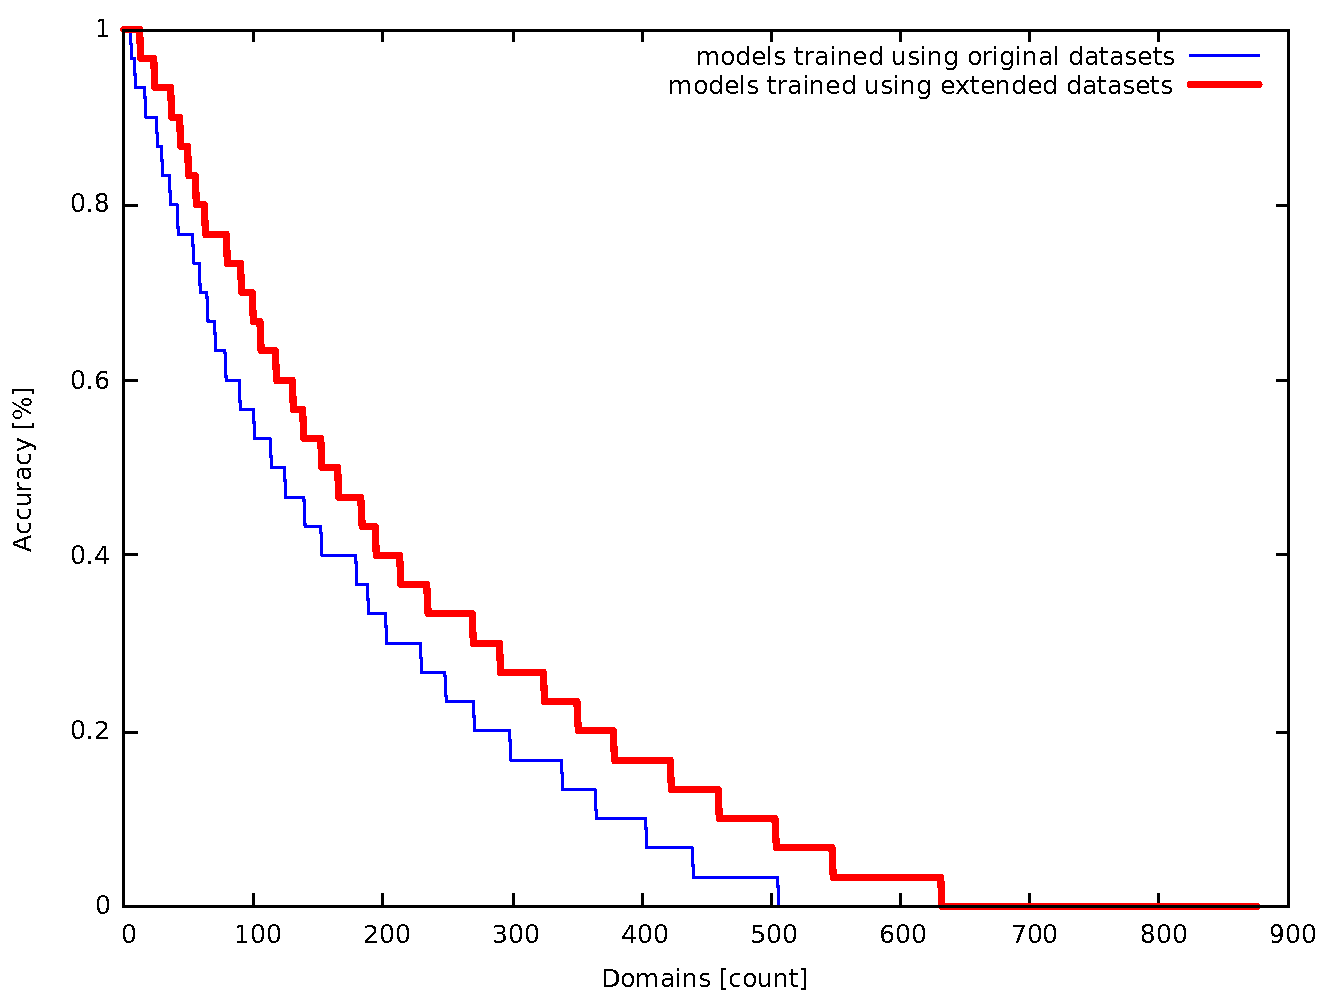
\includegraphics[width=1.0\textwidth]{plot_target_detection.pdf}
\end{figure}


\subsection{Results}
Total accuracy of the original model is 18 \%. Total accuracy of the extended model is 24 \%.
We can see that the extended model caused a significant performance increase in domain detection.
However 24\% accuracy cannot be generally considered a good result.

\footnotetext{Graph shows accuracy of detection for each domain. }

\par In order to make conclusions about performance of our domain detection solution we have to look at the distribution of the domains within the graph. This is important because we need to detect the domains that are common targets of the phishing attacks. Also it is not a problem if we cannot detect domains that are never attacked.
\par Figure \ref{table_target_detection} shows us a three samples from the distribution of the domains. 
We can see that sample of the most detected domains contains a lot of financial institutions. In contrast the sample of domains that were not detected at all contains mostly unknown domains or domains that are unlikely targets of the phishing attacks.

\par We examined the emails from the dataset and we have found out that some emails do not contain any mention of the targeted organization. This naturally lowers the performance achievable in this test.
\par Another thing that makes the domain detection hard is the number of domains we are trying to detect.

\par Because of observation we made we consider our domain target solution sufficient for our purposes.
We have proved that it is possible to improve domain detection performance by training better named entity recognized models.




\begin{figure}[!ht]
    \centering
    \caption[Target detection samples]{Target detection samples\protect\footnotemark }
    \label{table_target_detection}

\begin{tabular}{|l|l|l|l|}
\hline
80 \% and more &  around 55 \%  &  0 \% \\ \hline \hline
airbank.cz &  praha9.cz &  alza.cz \\ \hline
erasvet.cz &  totalbrokers.cz &  arcelormittal.com  \\ \hline 
itesco.cz &  berpujcku.cz &  babynabytek.cz \\ \hline 
realmoney.cz &  ceskapojistovna.cz &  boschrexroth.cz \\ \hline 
aaaauto.cz &  cez.cz &  canariatravel.cz \\ \hline 
ebay.com &  dracik.cz &  c-budejovice.cz \\ \hline 
ifortuna.cz &  eufrat.cz &  cement.cz \\ \hline 
zasilkovna.cz &  homecredit.cz &  ceskyserver.cz \\ \hline 
tchibo.cz &  paypal.com &  coleman.cz \\ \hline 
victoriatip.cz &  pns.cz &  e-rezervace.cz \\ \hline 
gigaserver.cz &  jtbank.cz &  fler.cz \\ \hline 
royalvision.cz &  sberbankcz.cz &  mendelu.cz \\ \hline 
slavia-pojistovna.cz &  agrofert.cz &  mora.cz \\ \hline 
equabank.cz &  hyundai.cz &  o2.cz \\ \hline 
vodafone.cz &  lr-czech.com &  pokrok.cz \\ \hline 
bohemiacargo.cz &  okgroup.cz &  prvni-lekarna.cz \\ \hline 
armexenergy.cz &  uvt.cz &  sam73.cz \\ \hline 
europ-assistance.cz &  ascari.cz &  sipkova.cz \\ \hline 
kbps.cz &  axa.cz &  spcr.cz \\ \hline 
reprofit.cz &  mall.cz &  vzp.cz \\ \hline 
\end{tabular}

\end{figure}
\footnotetext{We have randomly selected the same amount of domains for each column. Then we have picked the most interesting domains from each selected sample.}



\section{Phishing email detection}
We have successfully developed a targeted domain detection solution.
Next thing we had to do was developing a phishing detection solution that would allow us to evaluate the performance of the features based on the detected target. 


\subsection{Baseline solution}
We have implemented a baseline phishing email detection solution using python \cite{python}.
We have used random forest classifier implementation from the scikit-learn library. \cite{pySklearn} The classifier was configured to use 10 decision trees in the random forest.

\par For the baseline solution we chose 26 features. Features we used include all features listed in the features section \ref{features}. Some of the used features were taken from \cite{vitListik2015detekce}. 
 
\subsection{Testing baseline solution}
We have split the Email.cz dataset and used 20 \% of the data for testing. 
Accuracy achieved by the baseline solution using all available features was 97.6.

\par We have performed more tests using only one feature at the time. The three features with highest accuracy were number of phishing keywords, maximum number of periods in the URL and body richness.
\par Number of phishing keywords achieved 82.2 accuracy. Phishing keywords are predefined words that are characteristic for phishing emails.
\par Maximum number of periods in URL achieved 81.2 accuracy. It is interesting that such a simple feature can be so helpful for phishing email detection.
\par Body richness achieved 80.5 accuracy. This feature is defined in state of the art of this thesis \ref{bodyrichnes} section.



\section{Final solution}
Final solution was created by incorporating target based features into the baseline solution.
Target detection solution outputs an array of detected domains for each email.
Each domain in the array has an assigned probability that represents the likelihood of the domain being a target of the email.
\par Probability is determined by counting all entities in the email that can be mapped to the domain. Then the counts are normalized for all domains returned in the array so that the sum of all probabilities equals to 100 \%.

\subsection{Target based features}
Output from target detection was used to generate following features.
\par Domain detected feature is a boolean feature that is true if any domain was detected.
\par Top 1 detected domain feature which includes two values. First value is an id of the most probable detected domain. The second value is percentage that the domain is the target. 
\par Top 5 detected domains feature that is much like the top 1 feature. Except it includes percentages and id's for top 5 detected domains.
\par Last feature we have generated was boolean feature that detects mismatched links. Link is considered mismatched if it leads to domains that are not usually present in the emails sent by this specific target. Commonly linked domains are determined using historically collected data by Email.cz. We have implemented aggressive and benevolent versions for this feature. Both of these versions achieved similar performance and we will not differentiate between them from now on.


\subsection{Testing final solution} 
We have used the same testing data for both final solution and baseline solution testing.
Accuracy achieved by the final solution using all available features was 98. Which is a minor improvement over baseline solution with 97.7 accuracy. 

\par We have performed more tests using only one feature at the time. All three features with the highest accuracy were based on target detection. 
\par The three top features were: boolean domain detected feature, percentage for top 1 detected domain and link mismatch feature.
\par All three features achieved similar accuracy of 86.9. Compared to 82.2 accuracy for best feature from baseline solution.


\subsection{Results}
Testing showed us that target based features can improve the performance of the phishing emails detection.
We have found out that target based features provide a significant amount of information about an email.
Target based features outperform the commonly used features for phishing email detection.

\subsection{Possible improvements}

This thesis proves that Named entity recognition can be used for Czech phishing email detection.
However there is a lot of ways to improve the current solution. 

More data for Named entity recognition may be created.
New better Nametag models could be trained using created data.
This should improve to domain specific performance of the model.

Mapping is currently done using keyword and dictionary based approach.
This is not ideal because it depends on predefined data.
More methods for creating mappings should be researched.

Bigger phishing email dataset should be gathered to reduce the bias of the dataset.
Observations made in this thesis should be confirmed by testing using live traffic.

\setsecnumdepth{part}
\chapter{Conclusion}


We have researched the state of the art phishing email detection methods and the common methods of machine learning performance evaluation.
We have researched the state of the art Czech Named entity recognition system and the possibilities of using it to detect phishing attacks.

We have analyzed Nametag, the state of the art Czech Named entity recognition system. We managed to train models that match the performance of the original models \cite{stateOfTheArtCzechNER}.
Models for Nametag were trained using original datasets. The performance of the models was insufficient for our purpose because emails differ from structure of the original training data.
Domain specific performance have been improved by adding custom data to the original datasets. 

We have developed a solution that can predict the targeted organization of the phishing attack based on the Nametag output. 
We have used data from Phishtank \cite{phishtank} to test the accuracy of our solution. Models used for testing were trained using both original dataset and improved extended dataset. 

We have downloaded the list of the Czech subjects from ARES \cite{opendata_orgs}.
Firmy.cz \cite{firmycz}, the catalogue of Czech organizations, was used to get matching domains for downloaded subjects. 
We have developed a solution that maps recognized entities to domains using data from ARES and Firmy.cz.
Mappings for several important international banking and technology companies were added manually.
Czech dataset was extended using generated mappings and list of most attacked domains from Email.cz.
We have used legitimate emails from Email.cz dataset grouped by domain to evaluate performance of the solution.
Results of the testing showed the performance increase achieved by using the extended models.

We have developed a baseline phishing email detector using random forest classifier.
Features used for baseline solution were based on research of both English and Czech phishing detection solutions.
The performance of the baseline solution was measured.

Phishing target detection solution and domain mappings were used to generate features for phishing email detection.
Generated features were added to the baseline solution and the performance was evaluated.
Target based features caused a minor improvement in the total accuracy of the phishing detection solution. Accuracy achieved by the final solution with target based features was 98 compared to 97.7 accuracy achieved by baseline solution.

We have performed tests using only one feature at the time to discover the most significant features for phishing email detection.
The target based features achieved the best accuracy out of all used features. 
The top three most significant features were all based on target detection. These features achieve 86.9 accuracy when used as one feature at the time. For comparison the best feature from the baseline solution scored 82.2 accuracy.

These results suggest that target based features are powerful features for phishing email detection. 
Target based features improve the overall performance of the phishing email detection solution.
We are convinced that target based features are effective way to detect phishing emails.

More fine-tuning of the solution is a subject for future work. 
Further improvements may be achieved by improving various parts of the process such as Named entity recognition, target detection and domain mapping.
Phishing email detection solution itself could be improved by adding more target-based features or trying different machine learning methods.
Observations made in this thesis should be confirmed by testing using bigger dataset or live traffic.


\bibliographystyle{iso690}
\bibliography{mybibliographyfile}

\setsecnumdepth{all}
\appendix

\chapter{Acronyms}
\begin{description}
	\item[API] Application Programming Interface 
        \item[ARES] Administrativn{\' i} registr ekonomick{\' y}ch subjekt{\r u} (Administrational registry of economical subjects)
	\item[CNEC] Czech Named Entity Corpus
	\item[CoNLL] Conference on Computational Natural Language Learning
	%\item[DT] Decision trees
	\item[EML] Elecronic Mail
	\item[JSON] JavaScript Object Notation
	\item[MEMM] Maximum Entropy Markov Models
	\item[ML] Machine Learning
	\item[MUC] Message Understanding Conference
	\item[NER] Named Entity Recognition
	\item[NLP] Natural Language Processing
	\item[HMM] Hidden Markov Models
	\item[RAM] Random Access Memory
	\item[REST] Representational State Transfer
	%\item[RF] Random forest
	\item[RFC] Request for comments
	\item[URL] Uniform Resource Locator
\end{description}


\chapter{Contents of enclosed SD card}

\begin{figure}
	\dirtree{%
    	.1 data\DTcomment{the directory of data}.
        .2 feature\_data\DTcomment{the directory of extracted features for training}.
        .2 organizations\_data\DTcomment{the directory of organizations data}.
        .1 Makefile\DTcomment{Makefile for running selected parts of the implementation}.
        .1 readme.md\DTcomment{the file with SD card contents description}.
        .1 results\DTcomment{the directory with results of the training}.
        .1 src\DTcomment{the directory of source codes}.
        .2 code\DTcomment{implementation sources}.
        .3 addTargetFeatures.py\DTcomment{script for adding target based features}.
        .3 train.py\DTcomment{script for training the phishing email detector}.
        .3 more\DTcomment{more implementation sources}.
        .2 thesis\DTcomment{the directory of \LaTeX{} source codes of the thesis}.
        .1 text\DTcomment{the thesis text directory}.
        .2 thesis.pdf\DTcomment{the thesis text in PDF format}.
	}
\end{figure}

\end{document}
